% !TeX root = ../libro.tex
% !TeX encoding = utf8
\chapter{Desarrollo del simulador}
\section{Introducción}
Esta parte final está orientada a implementar los modelos y la resolución de sistemas de ecuaciones diferenciales como un servicio web (en el marco de arquitecturas orientadas a servicios o recursos) y hacer un simulador en una página web para mostrar la aplicación y utilidad de este trabajo de una forma mucho más gráfica y dinámica, pudiendo cambiar los parámetros del edificio a nuestro gusto y ver los resultados al instante.

Veremos el proceso y desarrollo del simulador, para el cual hemos utilizado tecnologías actuales que podremos encontrar en cualquier proyecto de desarrollo de las principales empresas, además veremos los aspectos más importantes en el proceso de creación del backend y frontend, mostraremos algunos ejemplos de casos de uso, además de unas posibles mejoras y actualizaciones que se podrían realizar sobre el proyecto a futuro.\\

El objetivo es que sea accesible para cualquier usuario, y para ello la interfaz será muy intuitiva y fácil de entender, además incluiremos al final una pequeña guía de instalación y acceso del simulador, de tal forma que cualquiera pueda utilizarlo y probarlo.
\section{Tecnologías utilizadas}
A continuación vamos a enumerar y explicar los principales motivos y características acerca de las tecnologías que hemos utilizado, empezando por las que hemos requerido para desarrollar el backend:
\begin{itemize}
	\item Python. Además de porque tiene una comunidad muy amplia, la cual nos permite encontrar feedback rápidamente sobre cualquier duda o problema que tengamos, es uno de los lenguajes más utilizados para ciencia de datos, IA y cálculo, por lo que existen muchas librerías para simplificar la implementación de nuestros sistemas de ecuaciones diferenciales.
	\item Flask. Es un framework utilizado comúnmente para crear aplicaciones web, y sobre todo, servicios web.
	\item JSON. Notación estándar para el intercambio de información entre los servicios y las aplicaciones.
	\item OpenAPI. Es una notación estándar para describir y compartir con otros usuarios (desarrolladores, comunidad) nuestro servicio web (resolución de sistemas de ecuaciones diferenciales).
\end{itemize}
En cuanto al desarrollo del frontend hemos utilizado:
\begin{itemize}
	\item React. Es una de las librerías más populares de JavaScript, está diseñada para crear interfaces de usuario con el objetivo de facilitar el desarrollo de aplicaciones en una sola página. Tiene un alto rendimiento y permite infundir código HTML con JavaScript. Aplicaciones muy populares como Facebook, Netflix, DropBox, Instagram o Paypal usan React, y es por ello que es tan importante y he querido familiarizarme con ella en este trabajo. Además, es mantenida por Facebook y la comunidad de software libre.
	\item Highcharts. Es una librería escrita en JavaScript para generar gráficos interactivos en aplicaciones web, soporta una gran variedad de gráficos y en nuestro caso la utilizaremos para mostrar el resultado final.
	\item Bootstrap. Es un framework que permite a los desarrolladores web darle forma a un sitio web y adaptarlo a las necesidades de los usuarios, nosotros lo hemos utilizado para mejorar el diseño de la página.
	\item Ant Design. Es una biblioteca React UI (User Interface), que como su nombre indica, permite construir interfaces de usuario con un elegante diseño, la hemos compaginado con Bootstrap para mejorar el diseño de la página.
\end{itemize}
\section{Desarrollo del Frontend}
El objetivo principal del frontend es tener una herramienta web, visual y atractiva, que mediante una serie de parámetros, nos permita obtener los valores correspondientes a la resolución de nuestros sistemas de ecuaciones diferenciales, para que cualquier tipo de usuario pueda hacer uso de esta herramienta sin tener un conocimiento experto relacionado con las matemáticas ni la informática.
\begin{figure}[h!]
	\centering
	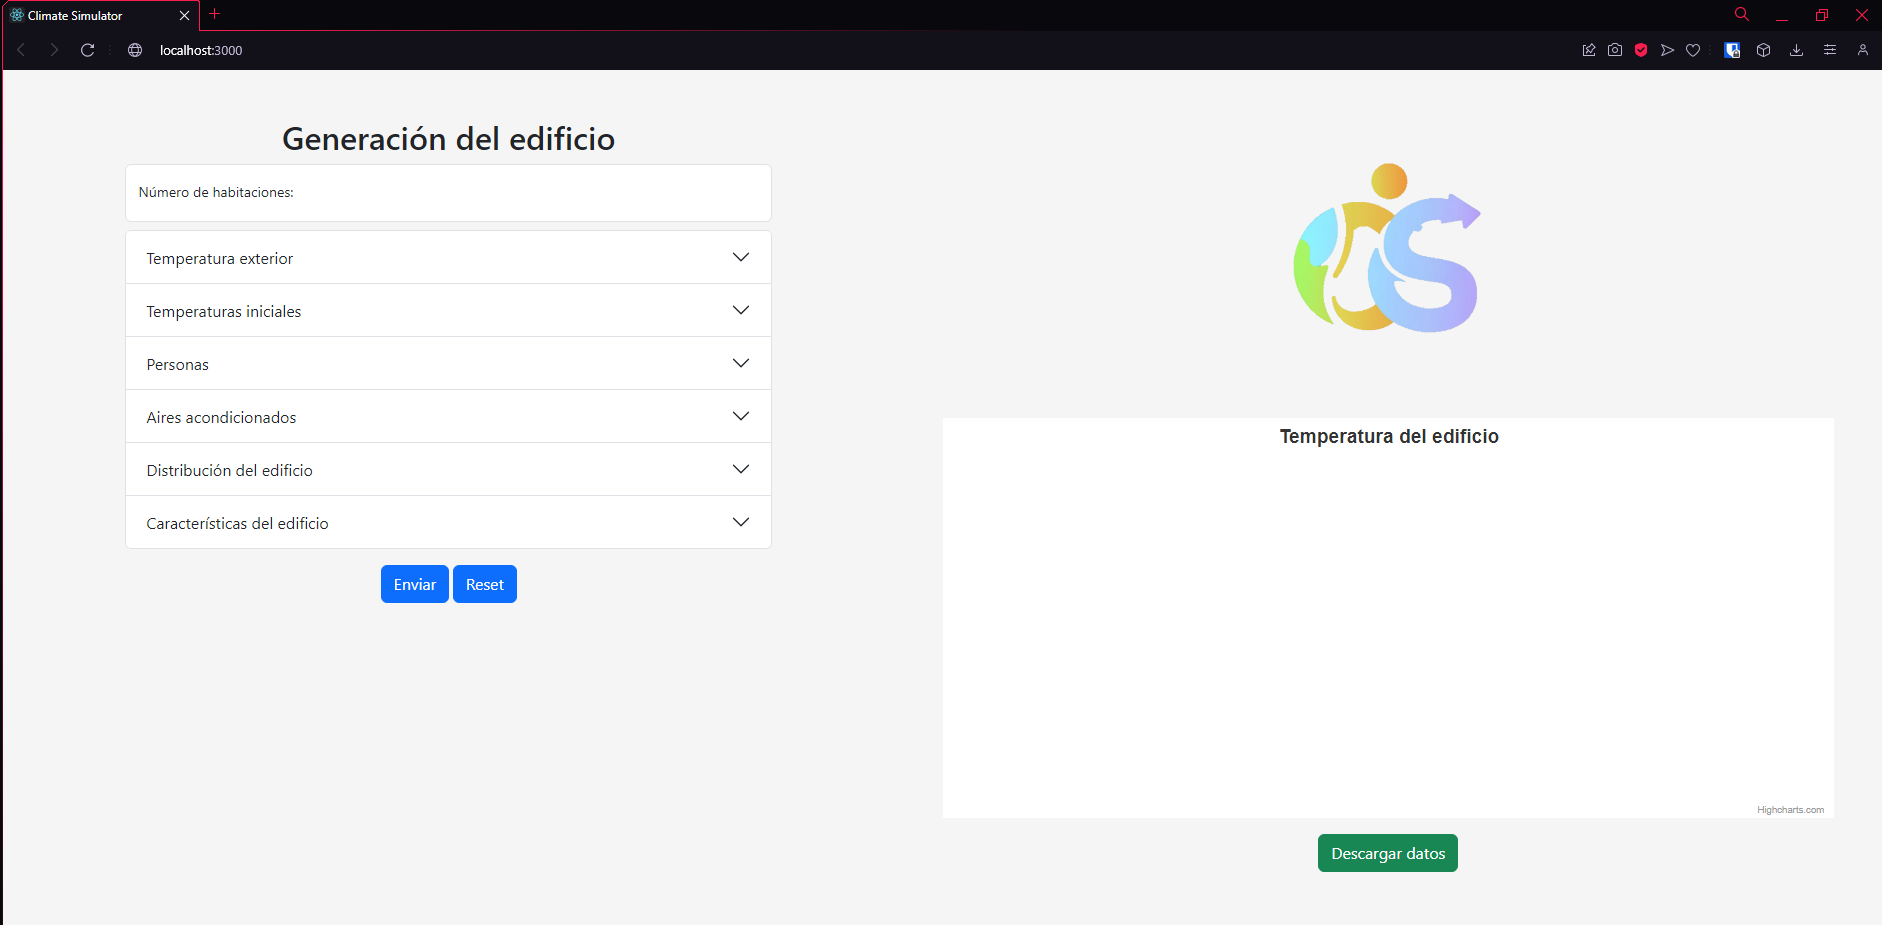
\includegraphics[width=\textwidth]{pag_web}
	\caption{Página web}
	\label{fig:pag_web}
\end{figure}

Nada más abrir la página nos encontramos con el aspecto que podemos ver en la \autoref{fig:pag_web}, donde a la izquierda tenemos un formulario dinámico que nos permite generar el edificio con todos los parámetros necesarios, y es que los campos del formulario varían en tiempo real según el número de habitaciones, esto es posible gracias a que estamos utilizando React. Para mejorar el diseño del formulario hemos utilizado tanto Ant Design como Bootstrap.
En la \autoref{fig:form_2habs} podemos ver cómo se incluyen 2 habitaciones en el desplegable al haber introducido que el edificio tendrá 2 habitaciones.
\begin{figure}[h!]
	\centering
	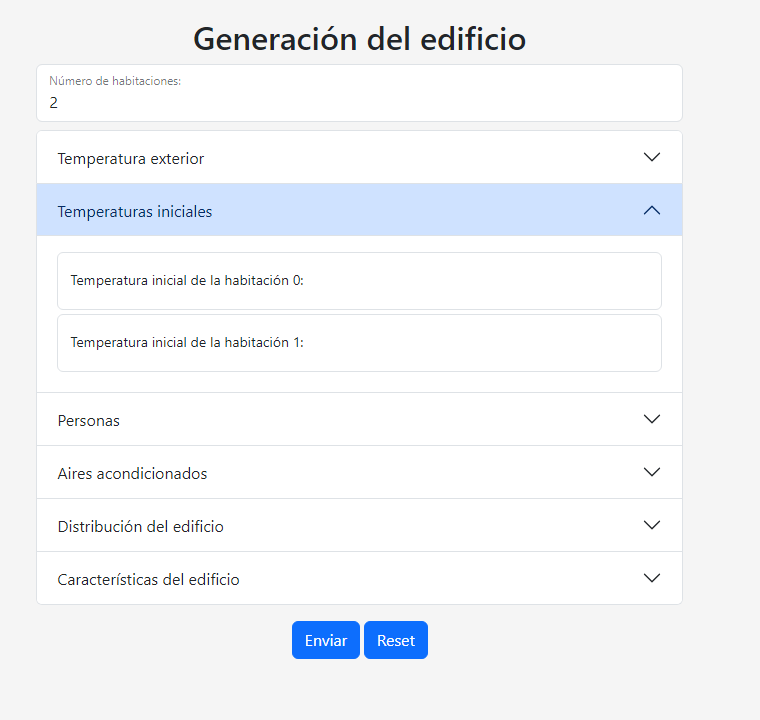
\includegraphics[width=0.8\textwidth]{formulario_2habs}
	\caption{Formulario introducir $2$ habitaciones}
	\label{fig:form_2habs}
\end{figure}
Para añadir la temperatura exterior, hemos incluido dos opciones, que podremos cambiar haciendo click en la barra superior del campo, como podemos ver en la \autoref{fig:temp_exterior}:
\begin{figure}[h!]
	\centering
	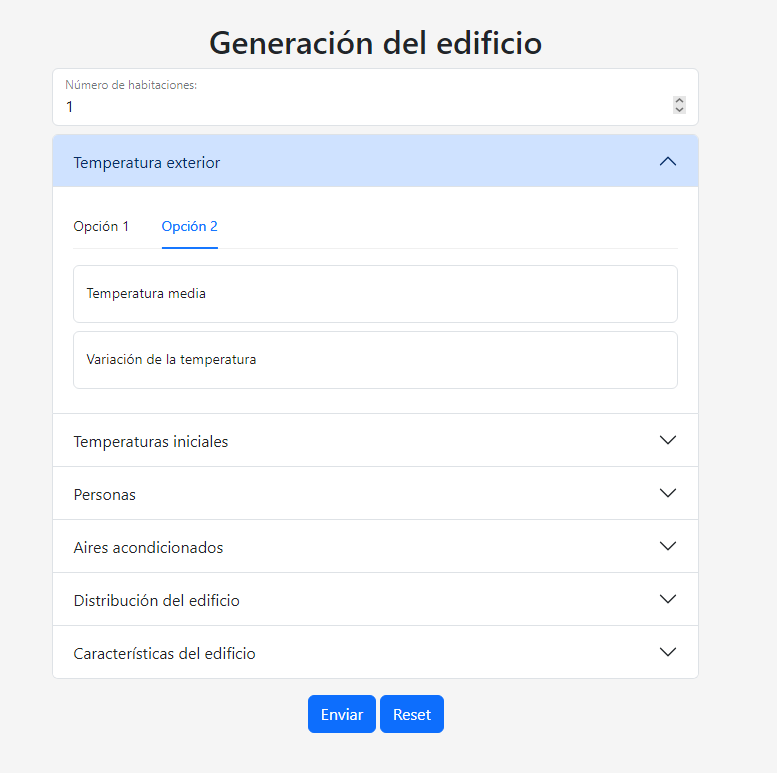
\includegraphics[width=0.8\textwidth]{temp_exterior}
	\caption{Opciones para la temperatura exterior}
	\label{fig:temp_exterior}
\end{figure}
\begin{figure}[h!]
	\centering
	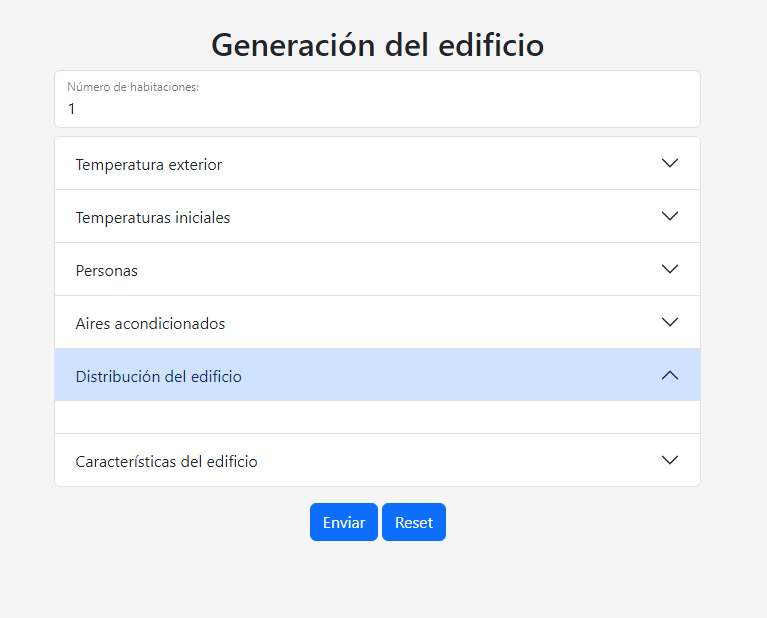
\includegraphics[width=0.8\textwidth]{una_hab}
	\caption{Formulario con $1$ habitación}
	\label{fig:una_hab}
\end{figure}
\begin{itemize}
	\item Opción $1$: Aquí podremos incluir directamente la función que tendrá la temperatura exterior durante las $24$ horas, está pensada para usuarios expertos en el tema. La función debe ser leída por la biblioteca $NumPy$ de Python, luego tendremos que usar expresiones como por ejemplo: $5 - 10*np.cos(t*np.pi/12)$
	\item Opción $2$: Podremos indicar la temperatura media del día y además cuánta variación tendrá, por ejemplo, si ponemos temperatura media de $10 \celsius$, y variación de $5$, entonces la temperatura variará entre $5 \celsius -15 \celsius$ grados, esta opción está pensada para que cualquier tipo de usuario pueda introducir la temperatura externa, sin necesidad de tener un conocimiento experto.
\end{itemize}

Otro detalle a tener en cuenta es que si ponemos sólo una habitación, no nos aparecerá la distribución del edificio, ya que no tendría sentido, como podemos ver en la \autoref{fig:una_hab}.

Al final tenemos dos botones tanto para enviar el formulario y obtener inmediatamente la gráfica con las temperaturas a la derecha, o para resetear el formulario por si queremos empezar de nuevo a crear el edificio.
\begin{figure}[h!]
	\centering
	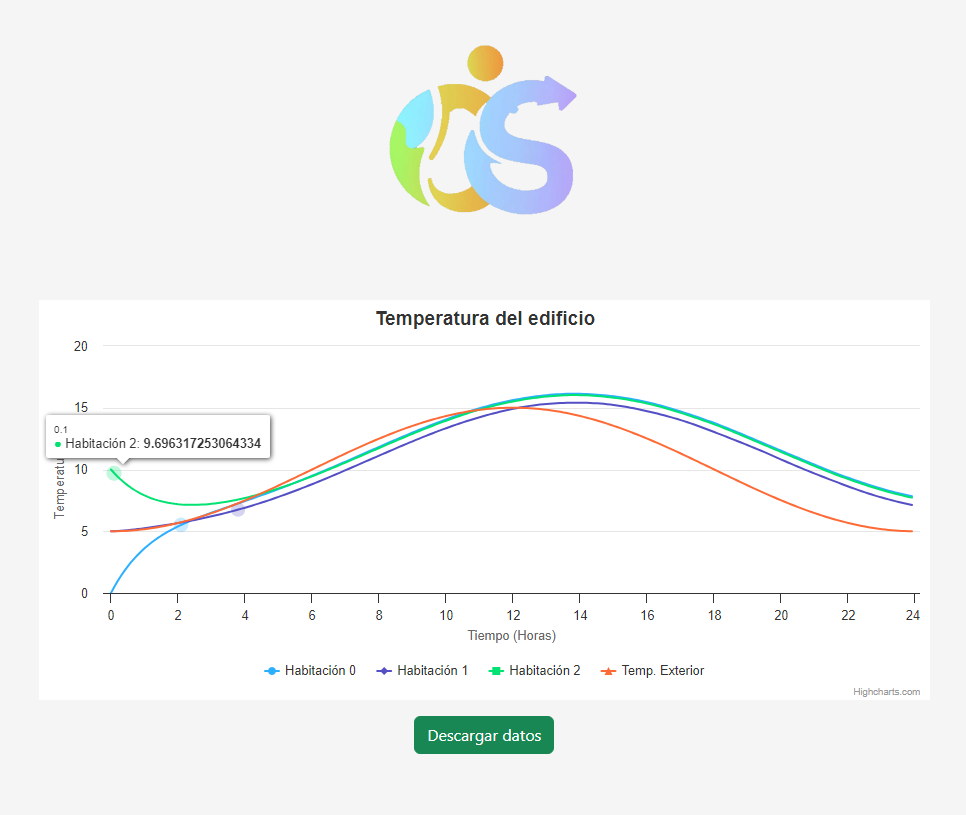
\includegraphics[width=\textwidth]{parte_derecha}
	\caption{Parte derecha de la página}
	\label{fig:parte_derecha}
\end{figure}
Ahora pasando a la parte derecha, tenemos en primer lugar el logo que hemos decidido añadir a la página, esto le aporta una identidad al proyecto aparte de ser más atractivo, justo debajo tenemos la solución al problema, es decir, una gráfica que hemos incluido gracias a Highcharts donde podemos ver las temperaturas de cada habitación, además de la temperatura externa para cada momento del día, y si pasamos el cursor por encima podemos ver el valor numérico de la temperatura en una hora determinada, todo esto se muestra en la \autoref{fig:parte_derecha}.

Por último, hemos incluido justo debajo un botón verde que nos permite descargar los datos de las temperaturas obtenidas en formato JSON, esta es una funcionalidad muy interesante que nos permite utilizar los resultados como posible entrada para otro programa por si fuesen necesarios.

\section{Desarrollo del Backend}
Vamos a utilizar un estilo RESTful, ya que es el más utilizado hoy en día, esto quiere decir que nuestro servicio web implementa una arquitectura de REST, que sirve para estandarizar comunicaciones web entre sistemas, logrando que se entiendan mucho mejor entre ellos. Se basa en que el cliente envía peticiones para recuperar o modificar recursos, y el servidor responde con el resultado, que puede ser con los datos que hemos pedido o el estado de la petición. ¿Incluir referencia por si se quiere encontrar más información acerca de las arquitecturas REST?
\begin{figure}[h!]
	\centering
	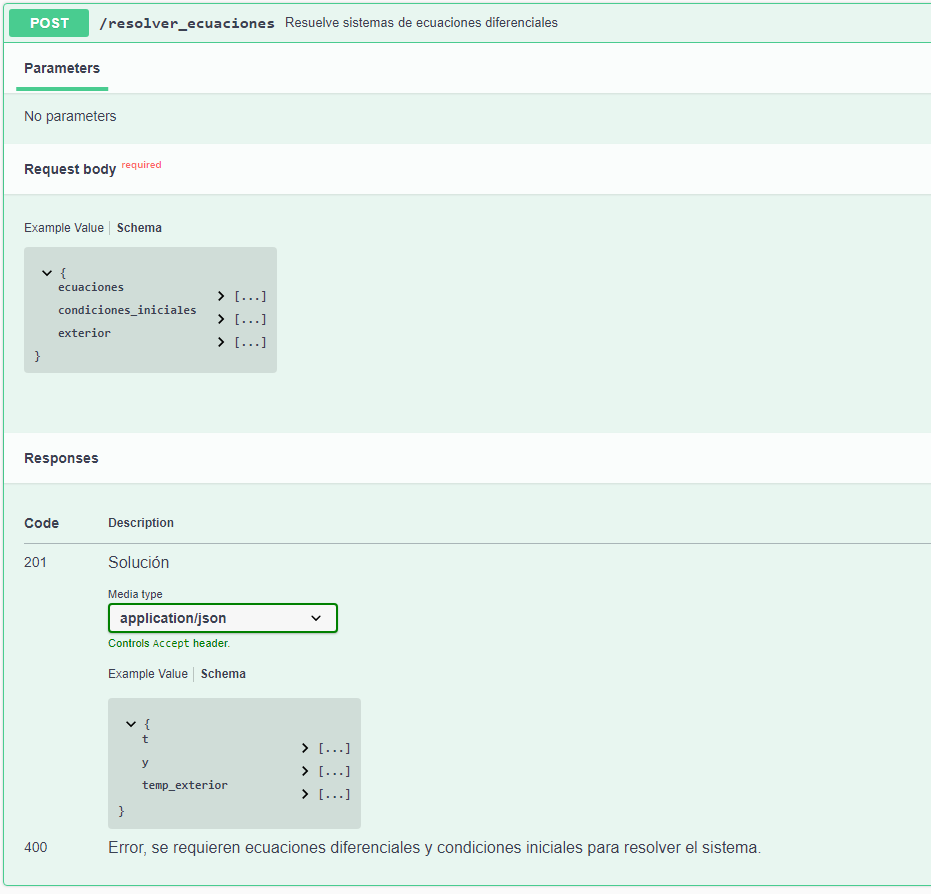
\includegraphics[width=\textwidth]{openapi}
	\caption{Especificación OpenAPI}
	\label{fig:openapi}
\end{figure}
Todo el desarrollo lo hemos realizado utilizando el lenguaje de programación Python, y nos hemos servido de Flask para crear el servicio web.

El objetivo principal de nuestra API es resolver sistemas de ecuaciones diferenciales, para ello recibimos del servidor web las ecuaciones, las condiciones iniciales y la función que representa la temperatura exterior del edificio, y devuelve un vector formado por:
\begin{itemize}
	\item Un vector con los puntos que representarán el tiempo en el eje $X$ (de $0$ a $24$ horas).
	\item Un vector en el que cada componente contiene otro vector con las temperaturas de cada habitación en cada instante de tiempo (los puntos del primer vector).
	\item Un último vector formado por la temperatura externa en cada instante de tiempo.
\end{itemize} 
Esto se lo mandamos como respuesta al frontend, donde se construirá la gráfica final con los resultados obtenidos.

Además, vamos a añadir el estándar de OpenAPI, que nos permite visualizar los métodos de la API para que cualquier programador o persona interesada pueda ver de forma esquemática el uso y funcionamiento detallado de cada uno de los métodos. Un detalle muy importante es que es independiente del lenguaje de programación con el que esté desarrollada la API. En la \autoref{fig:openapi} podemos ver cómo queda la documentación, la cual es accesible para todo el mundo.

\section{Casos de uso}
\subsection{Ejemplo con 3 habitaciones que vimos en la \autoref{fig:edif3}}
Siguiendo el modelo de edificio que tomamos en el ejemplo de la \autoref{fig:edif3}, vamos a rellenar el formulario con los siguientes datos:
\begin{itemize}
	\item Número de habitaciones: $3$
	\item Temperatura exterior: $5 - 10\cdot cos(t\cdot \pi/12)$
	\item Temperatura inicial de las habitaciones: $20,10,15$
	\item Cantidad de personas en las habitaciones: $1,10,0$
	\item Aires acondicionados en las habitaciones $0$ y $2$
	\item Distribución del edificio: 
	\begin{itemize}
		\item Habitaciones contiguas a la habitación $0$: $1,2$
		\item Habitaciones contiguas a la habitación $1$: $0$
		\item Habitaciones contiguas a la habitación $2$: $0$
	\end{itemize}
	\item Características del edificio:
	\begin{itemize}
		\item Constante de transferencia entre habitaciones: $5$
		\item Constante de transferencia con el exterior: $3$
		\item Calor generado por el aire acondicionado: $-8\celsius / 5h$
	\end{itemize}
\end{itemize}
Al introducir los datos en el formulario y hacer click en el botón Enviar, obtenemos la solución al problema, la cual coincide con la que vimos en \autoref{fig:graf_sol3}:
\begin{figure}[h!]
	\centering
	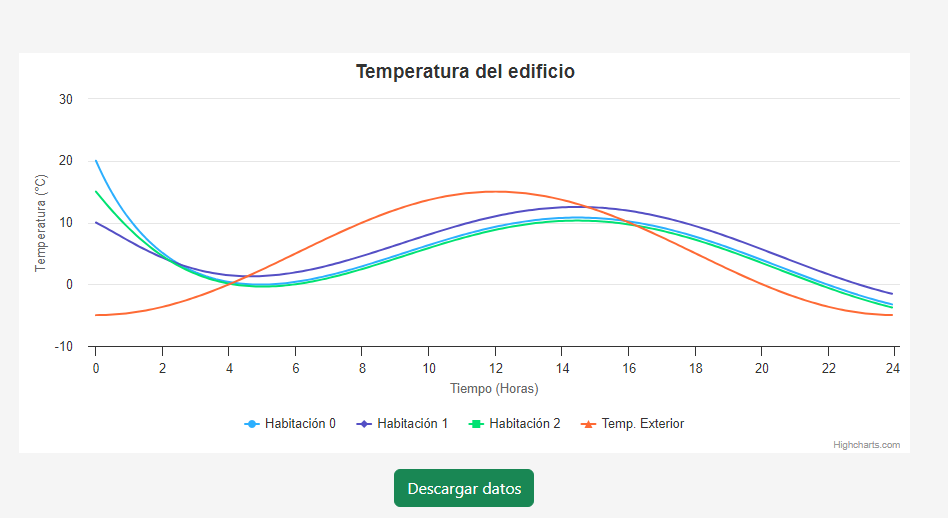
\includegraphics[width=\textwidth]{uso1}
	\caption{Temperaturas internas del edificio}
	\label{fig:caso1}
\end{figure}
\subsection{Ejemplo con 6 habitaciones}
Vamos a diseñar un nuevo edificio algo más elaborado, que constará de 6 habitaciones y seguirá la estructura que podemos ver en la \autoref{fig:edificio6}.
\begin{figure}[h!]
	\centering
	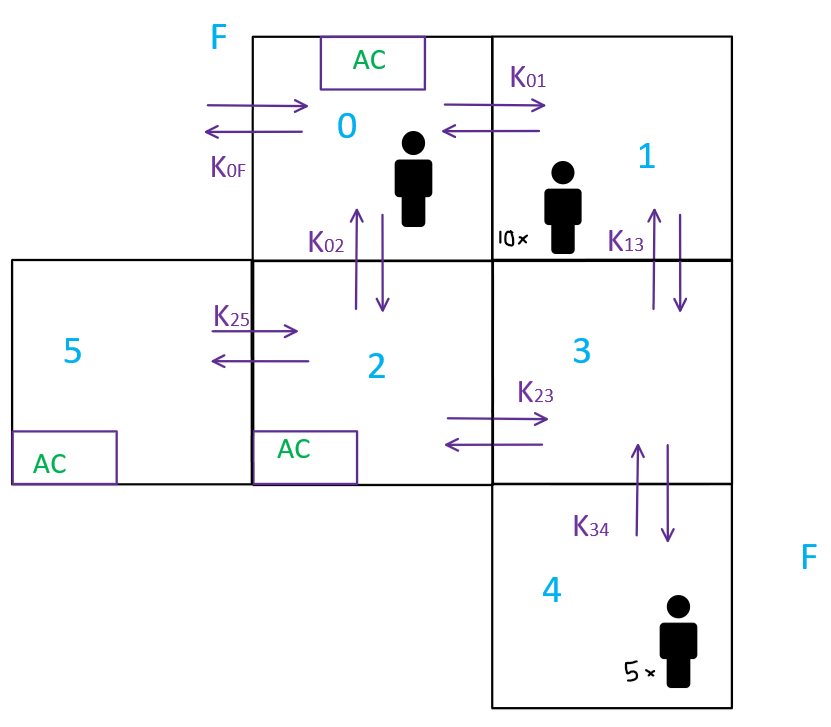
\includegraphics[width=0.8\textwidth]{edificio_6habs}
	\caption{Estructura del edificio con 6 habitaciones}
	\label{fig:edificio6}
\end{figure}
Vamos a introducir los siguientes datos en el formulario que corresponden con nuestro edificio:
\begin{itemize}
	\item Número de habitaciones: $6$
	\item Temperatura exterior: $20 - 15\cdot cos(t\cdot \pi/12)$
	\item Temperatura inicial de las habitaciones: $20,10,15,5,5,12$
	\item Cantidad de personas en las habitaciones: $1,10,0,0,5,0$
	\item Aires acondicionados en las habitaciones $0$, $2$ y $5$
	\item Distribución del edificio: 
	\begin{itemize}
		\item Habitaciones contiguas a la habitación $0$: $1,2$
		\item Habitaciones contiguas a la habitación $1$: $0,3$
		\item Habitaciones contiguas a la habitación $2$: $0,3,5$
		\item Habitaciones contiguas a la habitación $3$: $1,2,4$
		\item Habitaciones contiguas a la habitación $4$: $3$
		\item Habitaciones contiguas a la habitación $5$: $2$
	\end{itemize}
	\item Características del edificio:
	\begin{itemize}
		\item Constante de transferencia entre habitaciones: $3$
		\item Constante de transferencia con el exterior: $8$
		\item Calor generado por el aire acondicionado: $-4\celsius / h$
	\end{itemize}
\end{itemize}
Al introducir los datos en el formulario y hacer click en el botón Enviar, obtenemos la solución al problema, como podemos ver en la \autoref{fig:caso2}. Podemos observar que el edificio tiene un gran aislamiento con el exterior, y es por ello que las temperaturas de las habitaciones no se ven prácticamente influenciadas por la temperatura exterior, además de las altas temperaturas exteriores y tener un aire acondicionado que genera bastante frío, podríamos estar ante un escenario típico de verano.
\begin{figure}[h!]
	\centering
	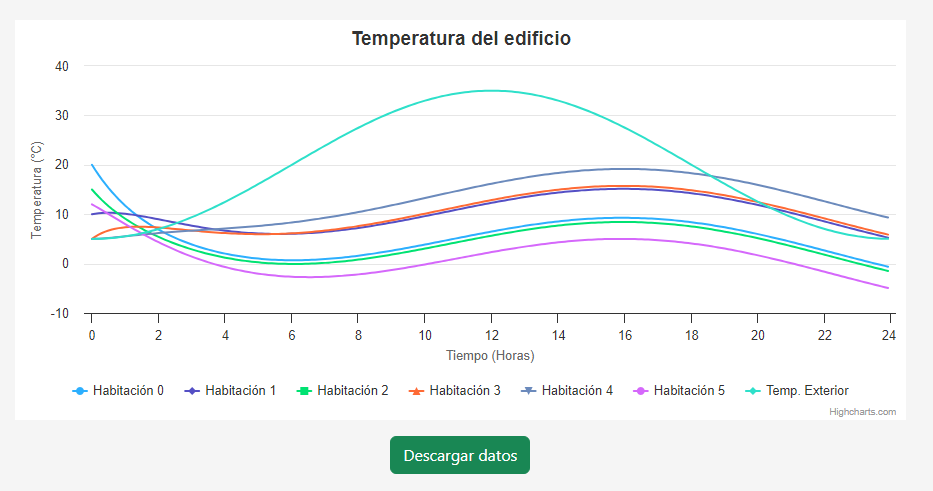
\includegraphics[width=\textwidth]{sol_6habs}
	\caption{Temperaturas internas del edificio con 6 habitaciones}
	\label{fig:caso2}
\end{figure}
\section{Actualizaciones y avances futuros}
Creando este proyecto me dí cuenta que se le podrían añadir unas mejoras y seguir trabajando en él a futuro, es decir, tenemos un proyecto escalable, algunas de las mejoras que se pueden añadir serían:
\begin{itemize}
	\item Cambiar la forma en la que se introducen los parámetros del edificio y hacer un panel en el que de forma gráfica y dinámica se vaya creando el edificio, y podamos ir añadiendo o quitando elementos tales como habitaciones, personas, etc... Esto sería una mejora en el diseño de la página además de permitir un uso más sencillo de la misma.
	\item Podríamos acceder a una API de tiempo meteorológico para no tener que introducir la temperatura externa a mano y obtenerla automáticamente. Además de trabajar con las próximas $24$ horas, podríamos estudiar cualquier día o intervalo de tiempo en específico.
\end{itemize}
\section{Manual de instalación y acceso}
\subsection{Requisitos previos}
Antes de instalar y ejecutar el programa, debemos tener instalado lo siguiente en el sistema:
\begin{itemize}
	\item Python
	\item PIP (gestor de paquetes de Python)
	\item Flask, NumPy, SciPy, Flask-CORS (librerías de Python)
	\item npm y Node.js
	\item React
\end{itemize}
\subsection{Instrucciones de instalación}
\subsubsection{Primera parte: API}
\begin{enumerate}
	\item Clonamos el repositorio del TFG desde GitHub y accedemos al de la API:
	\begin{verbatim}
		git clone https://github.com/vaynilla/TFG.git
		cd API_TFG
	\end{verbatim}
	\item Instalamos las dependencias de Python utilizando PIP:
	\begin{verbatim}
		pip install -r requirements.txt
	\end{verbatim}
	\item Ejecutamos el servidor de la API:
	\begin{verbatim}
		python app.py
	\end{verbatim}
	La API ahora debería estar en funcionamiento y accesible en la dirección URL especificada (por ejemplo, http://localhost:$5000$).
\end{enumerate}
\subsubsection{Segunda parte: Simulador}
\begin{enumerate}
	\item Accedemos al repositorio del simulador:
	\begin{verbatim}
		cd simulador
	\end{verbatim}
	\item Instalamos las dependencias del proyecto utilizando npm:
	\begin{verbatim}
		npm install
	\end{verbatim}
	\item Iniciamos la aplicación:
	\begin{verbatim}
		npm start
	\end{verbatim}
\end{enumerate}
\subsubsection{Acceso a la aplicación}
Una vez hemos completado los pasos anteriores, podremos acceder a la aplicación desde el navegador web:
\begin{itemize}
	\item Backend (API): La API estará disponible en la URL especificada por Flask (por ejemplo, http://localhost:$5000$).
	\item Frontend (React): La aplicación frontend estará disponible en http://localhost:$3000$ por defecto, a menos que se especifique lo contrario.
\end{itemize}




\endinput
%------------------------------------------------------------------------------------
% FIN DEL CAPÍTULO. 
%----------------------------------------------------------------------------------
-